\section{Durchführung}
\label{sec:Durchführung}
\subsection{Aufbau des Prismen-Spektralapparates}

\begin{figure}
  \centering
  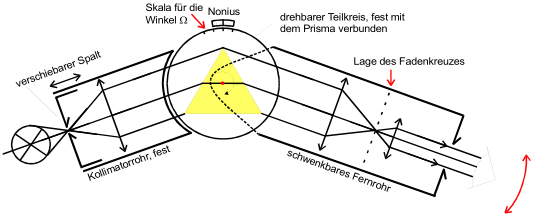
\includegraphics[scale=0.7]{images/Aufbau.png}
  \caption{Der Aufbau des verwendeten Prismen-Spektralapparates: Aus der Anleitung des Versuches \cite[24]{1}}
  \label{fig:aufbau}
\end{figure}

Um die Dispersionskurve des Materiales eines Prismas zu bestimmen, wird ein Prismen-Spektralapparat verwendet.
Dieser leitet den Lichtstrahl einer Cadmium-Quecksilber-Dampflampe über ein Kollimatorrohr durch das zu untersuchende Prisma.
Dort wird er zweimal gebrochen und bei richtiger Einstellung von einem drehbar befestigten Fernglas aufgefangen.
Um die richtige Kalibrierung zu ermöglichen ist das Prisma auf einem drehbaren Tisch fixiert und verfügt über ein Fadenkreuz.
Das Fernglas und der drehbare Tisch bilden ein Goniometer und ermöglichen damit eine präzise Winkelmessung.
Der schematische Aufbau kann der Abbildung \ref{fig:aufbau} entnommen werden.

\subsection{Messung des \texorpdfstring{$\upvarphi$}{phi}-Winkels}

\begin{figure}[H]
  \centering
  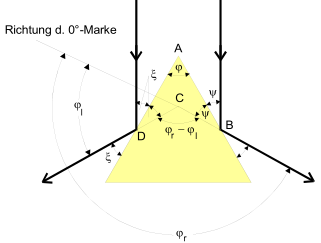
\includegraphics[scale=0.6]{images/Phi.png}
  \caption{Ausrichtung des Prismas für die $\upvarphi$-Messung: Aus der Anleitung des Versuches \cite[26]{1}}
  \label{fig:Phi}
\end{figure}

Um den Winkel $\phi$ zu bestimmen, muss das Prisma mit seiner reflektierenden Kante auf das Kollimatorrohr ausgerichtet werden.
Dies ist schematisch in Abbildung \ref{fig:Phi} dargestellt.
Das Licht wird somit an zwei der Prismenoberflächen gebrochen.
Das Prisma wird fixiert, so dass sich die $\SI{0}{\degree}$-Marke nicht verändern kann.
Nun wird das Fernglas so gedreht, dass der Lichtstrahl einer Oberfläche im Fadenkreuz liegt.
Der Winkel wird gemessen und der Vorgang für die gegenüberliegende Seite wiederholt.
Diese Messungen werden jeweiles sieben mal durchgeführt.

\subsection{Messung des \texorpdfstring{$\eta$}{eta}-Winkels}

\begin{figure}
  \centering
  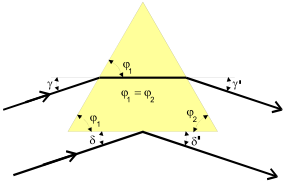
\includegraphics[scale=0.6]{images/Eta.png}
  \caption{Der gesuchte parallele Strahlengang: Aus der Anleitung des Versuches \cite[26]{1}}
  \label{fig:Eta}
\end{figure}

Um den Winkel $\eta$ bestimmen zu können, muss ein paralleler Strahlengang hergestellt werden.
Ein Teil des Lichtes aus dem Kollimatorrohr fällt Lichtes auf die Oberfläche des Prismas und wird dort reflektiert, während der andere Teil des Lichtes im Prisma gebrochen wird.
Es entsteht ein paralleler Strahlengang, welcher in Abbildung \ref{fig:Eta} dargestellt wurde.
Nun ist sowohl das Spektrum der Cadmium-Quecksilber-Dampflampe, als auch der reflektierte Lichtstrahl sichtbar.
Durch Drehen des Tisches, auf dem das Prisma ruht, und des Fernrohrs wird der Lichtstrahl mit den Spektrallinien in Deckung gebracht.
Der entsprechende Winkel wird notiert und der Vorgang für alle Spektrallinien wiederholt.
Danach wird der Prisma gemäß Abbildung \ref{fig:Drehung} rotiert und die Messungen für die gegenüberliegeden Seite durchgeführt.
Zu Beachten ist hierbei, dass die $\SI{0}{\degree}$-Marke mitgeschwenkt wird.

\begin{figure}
  \centering
  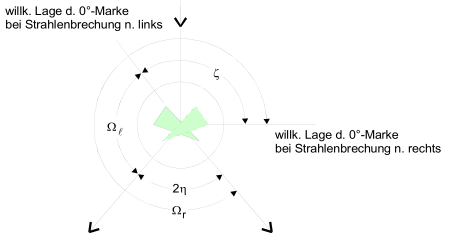
\includegraphics[scale=0.6]{images/Drehung.png}
  \caption{Darstellung der Rotation des Prismas: Aus der Anleitung des Versuches \cite[25]{1}}
  \label{fig:Drehung}
\end{figure}
